

%----------------------------------------------------------------------------------------
%	PACKAGES AND OTHER DOCUMENT CONFIGURATIONS
%----------------------------------------------------------------------------------------

\documentclass[12pt, oneside]{Thesis} % The default font size and one-sided printing (no margin offsets)

\graphicspath{{Pictures/}} % Specifies the directory where pictures are stored

\usepackage[square, numbers, comma, sort&compress]{natbib} % Use the natbib reference package - read up on this to edit the reference style; if you want text (e.g. Smith et al., 2012) for the in-text references (instead of numbers), remove 'numbers' 
\hypersetup{urlcolor=blue, colorlinks=true} % Colors hyperlinks in blue - change to black if annoying
\title{\ttitle} % Defines the thesis title - don't touch this

\usepackage{mathptmx, imakeidx,tfrupee, hyperref,listings,color,textcomp,algorithm, pdfpages, setspace,imakeidx, datetime, ragged2e, enumitem}

%\usepackage{fontspec}   Compile with XeLaTeX or LuaLaTeX
%\setmainfont{Times New Roman} Freeman E.

\makeindex

\hypersetup{%
	colorlinks=true,% Colour links without boxes
	linkcolor=black}% Internal link colour is black

\usepackage[noend]{algpseudocode}% http://ctan.org/pkg/algorithmicx
\algrenewcommand\Return{\State \algorithmicreturn{} }%


\definecolor{listinggray}{gray}{0.9}
\definecolor{lbcolor}{rgb}{0.9,0.9,0.9}
\lstset{
	backgroundcolor=\color{lbcolor},
	tabsize=4,
	rulecolor=,
	language=matlab,
	basicstyle=\scriptsize,
	upquote=true,
	aboveskip={1.5\baselineskip},
	columns=fixed,
	showstringspaces=false,
	extendedchars=true,
	breaklines=true,
	prebreak = \raisebox{0ex}[0ex][0ex]{\ensuremath{\hookleftarrow}},
	frame=single,
	showtabs=false,
	showspaces=false,
	showstringspaces=false,
	identifierstyle=\ttfamily,
	keywordstyle=\color[rgb]{0,0,1},
	commentstyle=\color[rgb]{0.133,0.545,0.133},
	stringstyle=\color[rgb]{0.627,0.126,0.941},
}

\makeindex[intoc]

%\usepackage{draftwatermark}
%\SetWatermarkText{Sample}




\begin{document}
	
% All the Variable should be entered inside {}
% If not applicable leave empty {} do not delete {}.

% Name of the University
\newcommand{\UniversityName}
{CHRIST (Deemed to be University)}


% Title of the project or thesis in capital letters
\newcommand{\ProjectTitle}
{Cosmic-Zoom}


% Title of the project or thesis in title case
\newcommand{\ProjectTitleTwo}
{Cosmic-Zoom}


% Type of Dissertation M.Tech Dissertation or B.Tech Dissertation
\newcommand{\DissertationType}
{A Project Report on}

% Program name: MASTER OF TECHNOLOGY or BACHELOR OF TECHNOLOGY in Uppercase
\newcommand{\ProgramNameUpper}
{BACHELOR OF TECHNOLOGY}

% Program name: Master of Technology or Bachelor of Technology in Normal case
\newcommand{\ProgramName}
{Bachelor of Technology}

% Program Short form: M.Tech. or B.Tech.
\newcommand{\ProgramNameShort}
{B.Tech.}


% Specialization: 
% For B.Tech : Electrical and Electronics Engineering, Mechanical Engineering 
% For M.Tech : Power Systems, VLSI Design, Software Engineering
\newcommand{\SpecializationName}
{Computer Science and Engineering}


% Name of Student in the Alphabetical Order should be written in {} for each. Leave blank braces for other Author name if it is individual project
% 
\newcommand{\AuthorNameOne}
{Ram Shankar Choudhary}

\newcommand{\RegisterNoOne}
{(1760357)}

\newcommand{\AuthorDepartmentOne}
{Computer Science \& Engineering}


\newcommand{\AuthorNameTwo}
{ }

\newcommand{\RegisterNoTwo}
{ }

\newcommand{\AuthorDepartmentTwo}
{ }


\newcommand{\AuthorNameThree}
{ }

\newcommand{\RegisterNoThree}
{ }

\newcommand{\AuthorDepartmentThree}
{ }


\newcommand{\AuthorNameFour}
{ }

\newcommand{\RegisterNoFour}
{ }

\newcommand{\AuthorDepartmentFour}
{ }


% Name of the Guide
\newcommand{\GuideName}
{Dr. Sandeep Kumar}

% Designation of the Guide
\newcommand{\GuideDesignation}
{Associate Professor}

% Department of Guide where he belongs to
\newcommand{\GuideDepartment}
{Guide Department}


% Name of the Co-Guide
\newcommand{\CoGuideName}
{Samhitha Kottamasu}

% Designation of the Co-Guide
\newcommand{\CoGuideDesignation}
{Exhibition Coordinator }

% Department of Co-Guide where he belongs to
\newcommand{\CoGuideDepartment}
{}


% 1. Give first author name and generate report
% 2. Take print out of only this sheet
%.3. Repeat this for all the authors
% 4. Keep this in the individual copy and bind the report
\newcommand{\NameofAuthortobeCertified}
{Ram Shankar Choudhary}


% Address of the department where project offically executed
\newcommand{\DepartmentNameAddress}
{ %\renewcommand{\baselinestretch}{1.0}
\textbf{\large{
	Department Name\\ 
	\CollegeName, \\ \UniversityName,\\ 
	Kumbalagudu,\,Bengaluru\,-\,560~074
}}

} 


% Project Date in month-yyyy format
\newcommand{\ProjectDate}
{May-2021}

% Academic Year in yyyy-yyyy format
\newcommand{\AcademicYear}
{2020-2021}

% Name of the department only
\newcommand{\DepartmentName}
{Department Name}

% Name of the College
\newcommand{\CollegeName}
{School of Engineering and Technology}


% Name of the HOD or Coordinator
\newcommand{\HODorCoordinator}
{Dr. K Balachandran}

% Name of the Position of the Head. eg: Head of the Department, Coordinator
\newcommand{\HODorCoordinatorDesignation}
{Head of the Department}


% Name of the Vice-Chancellor
\newcommand{\VCName}
{Dr. Rev. Fr. Abraham V M}

% Name of the Pro Vice Chancellor
\newcommand{\ProVCName}
{Dr. Rev. Fr. Joseph CC}

% Name of the Director of the College
\newcommand{\DirectorName}
{Dr. Fr. Benny Thomas}

% Name of the Dean/Associate Dean
\newcommand{\DeanName}
{Dr. Iven Jose}

% Name of the Position of Dean/Associate Dean
\newcommand{\DeanDesignation}
{Dean}

% If the project work done by more than one student then 'We' in side {} or 'I' if individual project 
\newcommand{\WeorI}
{We}

% Acknowledgement for Guide
\newcommand{\AcknowledgementForGuide}
{
	\WeorI~also extremely grateful to my guide, \textbf{\GuideName}, who has supported and helped to carry out the project. His constant monitoring and encouragement helped me keep up to the project schedule.
}

% Acknowledgement for Co-Guide(Leave blank if no co-guide) 
\newcommand{\AcknowledgementForCoGuide}
{
	\WeorI~also extremely grateful to my co-guide, \textbf{\CoGuideName}, who has supported and helped to carry out the project. His constant monitoring and encouragement helped me keep up to the project schedule.
}


% Acknowledgement for Others
\newcommand{\AcknowledgementForOthers}
{
	If outside the college-mention the organisation and the concerned people, like head of the organisation, guide and any other person you want to thank. All faculty and non-teaching staff. You may acknowledge your parents or any who supported you.
}

% Date of Declaration

\newcommand{\DateofDeclaration}
{15-06-2021}


\frontmatter % Use roman page numbering style (i, ii, iii, iv...) for the pre-content pages

\setstretch{1.5} % Line spacing of 1.3

% Define the page headers using the FancyHdr package and set up for one-sided printing
\fancyhead{} % Clears all page headers and footers
\rhead{\thepage} % Sets the right side header to show the page number
\lhead{} % Clears the left side page header

\pagestyle{fancy} % Finally, use the "fancy" page style to implement the FancyHdr headers

\newcommand{\HRule}{\rule{\linewidth}{0.5mm}} % New command to make the lines in the title page

% PDF meta-data
\hypersetup{pdftitle={\ProjectTitle}}
\hypersetup{pdfsubject=\SpecializationName}
\hypersetup{pdfauthor=\AuthorNameOne}
\hypersetup{pdfkeywords=\GuideName \\ \DepartmentName}

%----------------------------------------------------------------------------------------
%	TITLE PAGE
%----------------------------------------------------------------------------------------


\begin{titlepage}
	
\begin{center}
		\begin{figure}[!hb]
			\centering {{
\includegraphics[totalheight=1.4in]{cufe_logo.jpg}}}
		\end{figure}
	{\Large{\DissertationType}} \\
	\vspace{0.2in}
	{\large \textbf{\textrm{\ProjectTitle}}}\\
	\vspace{0.2in}%{1cm}
	{Submitted in partial fulfillment of the requirements
	for the degree of }\\

	{\large{{\textbf{\textrm{ \ProgramNameUpper\\}}}}}

	{\large{{\textbf{\textrm{in\\}}}}}
	
	{\large{{\textbf{\textrm{ \SpecializationName\\}}}}}

	{\large{by}}\\

	\begin{tabular}{cc}
%					{\large{\textrm{\textbf{Name}}}} & {\large{~Register Number}}\\
%					\hline
			{\large{\textrm{\textbf{\AuthorNameOne}}}} & {\large{~\RegisterNoOne}}\\
			{\large{\textrm{\textbf{\AuthorNameTwo}}}} & {\large{~\RegisterNoTwo}}\\
			{\large{\textrm{\textbf{\AuthorNameThree}}}} & {\large{~\RegisterNoThree}}\\
			{\large{\textrm{\textbf{\AuthorNameFour}}}} & {\large{~\RegisterNoFour}}\\

	\end{tabular}

	\vspace{0.1cm}
	

	\vspace{0.5cm}
	{\large{Under the Guidance of}}\\
	\vspace{0.1cm} {\large{\textrm{\textbf{\GuideName}\\
				\ifdefempty{\CoGuideName}{}{\vspace{-0.1in} {\normalsize and} \\ {\textbf{\CoGuideName}}}
				}}} \vspace{0.20cm}
\ifdefempty{\CoGuideName}{\vspace{0.3in}}{}	

		\DepartmentNameAddress 
	\ProjectDate
\end{center}

\end{titlepage}

\clearpage



\fancyhead[]{}
\renewcommand\footrulewidth{0pt}
\renewcommand\headrulewidth{0pt} 

\fancypagestyle{plain}{
	\fancyhead{}
	\fancyfoot[R]{\thepage}
}

%----------------------------------------------------------------------------------------
%	Certificate Page
%----------------------------------------------------------------------------------------

\newpage
\certificate{
\begin{center}
		\begin{figure}[!hb]
			\centering {{
\includegraphics[totalheight=1.4in]{cufe_logo.jpg}}}
		\end{figure}

		\textbf{{\LARGE{{\textrm{ \CollegeName\\}}}}}

		{\Large{{\textrm{ \DepartmentName\\}}}}
			\vspace{0.5in}
		{\Large \textbf{\textrm{CERTIFICATE}}}\\
\end{center}		
		\justify
		{
		This is to certify that \textbf{\NameofAuthortobeCertified} has successfully completed the project work entitled~\textquotedblleft\textbf{\ProjectTitleTwo}\textquotedblright~in partial fulfillment for the award of \textbf{\ProgramName} in \textbf{\SpecializationName} during the year \textbf{\AcademicYear}.
	}
\begin{center}		
	\begin{tabular}{p{5cm} p{2cm} p{5cm}}
			\vspace{0.5cm} &  \\
		\textbf{\GuideName}&&\ifdefempty{\CoGuideName}{}{\textbf{\CoGuideName}} \\
		\GuideDesignation&&\ifdefempty{\CoGuideName}{}{\CoGuideDesignation} \\
			\vspace{0.5cm} & &\\
		\textbf{\HODorCoordinator}&&\textbf{\DeanName} \\
		\HODorCoordinatorDesignation&&\DeanDesignation\\
	\end{tabular}
\end{center}

}

\clearpage


%----------------------------------------------------------------------------------------
%	Bonafide Certificate Page
%----------------------------------------------------------------------------------------

\newpage
\BonafideCertificate{
\begin{center}
		\begin{figure}[!hb]
			\centering {{
\includegraphics[totalheight=1.4in]{cufe_logo.jpg}}}
		\end{figure}

		\textbf{{\LARGE{{\textrm{ \CollegeName\\}}}}}

		{\Large{{\textrm{ \DepartmentName\\}}}}
			\vspace{0.5in}
		{\Large \textbf{\textrm{BONAFIDE CERTIFICATE}}}\\
\end{center}		
		
		\justify
		{
		It is to certify that this project titled~\textquotedblleft\textbf{\ProjectTitleTwo}\textquotedblright~is the bonafide work of
	}
	
	\begin{center}
		\begin{tabular}{p{4cm}lp{6cm}}
			\hline
			{\large{\textrm{\textbf{Name}}}} & {\large{\textbf{Register Number}}} & {\large{~\textbf{Department}}}
			\\
			\hline
			{\large{\textrm{\textbf{\AuthorNameOne}}}} & {\large{\RegisterNoOne}} & {\large{\AuthorDepartmentOne}} \\
			{\large{\textrm{\textbf{\AuthorNameTwo}}}} & {\large{\RegisterNoTwo}} & {\large{\AuthorDepartmentTwo}}\\
			{\large{\textrm{\textbf{\AuthorNameThree}}}} & {\large{\RegisterNoThree}} & {\large{\AuthorDepartmentThree}}\\
			{\large{\textrm{\textbf{\AuthorNameFour}}}} & {\large{\RegisterNoFour}} & {\large{\AuthorDepartmentFour}}
			
		\end{tabular}
	\end{center}
	\begin{tabular}{p{6cm} p{0.25cm} p{5cm}}
		
		\textbf{Examiners [Name and Signature]}&& Name of the Candidate :\\
		1.&& Register Number           : \\
		&&Date of Examination     : \\
		&& \\
		2.&& \\

	\end{tabular}



}



%----------------------------------------------------------------------------------------
%	Certificate Page (Comment if project is not done in industry)
%----------------------------------------------------------------------------------------



\IndustryCertificate{

	\pagestyle{empty}
	\begin{center}
		
		\begin{figure}[H]
			\begin{center}
				\centering
				\hspace*{-3cm}
				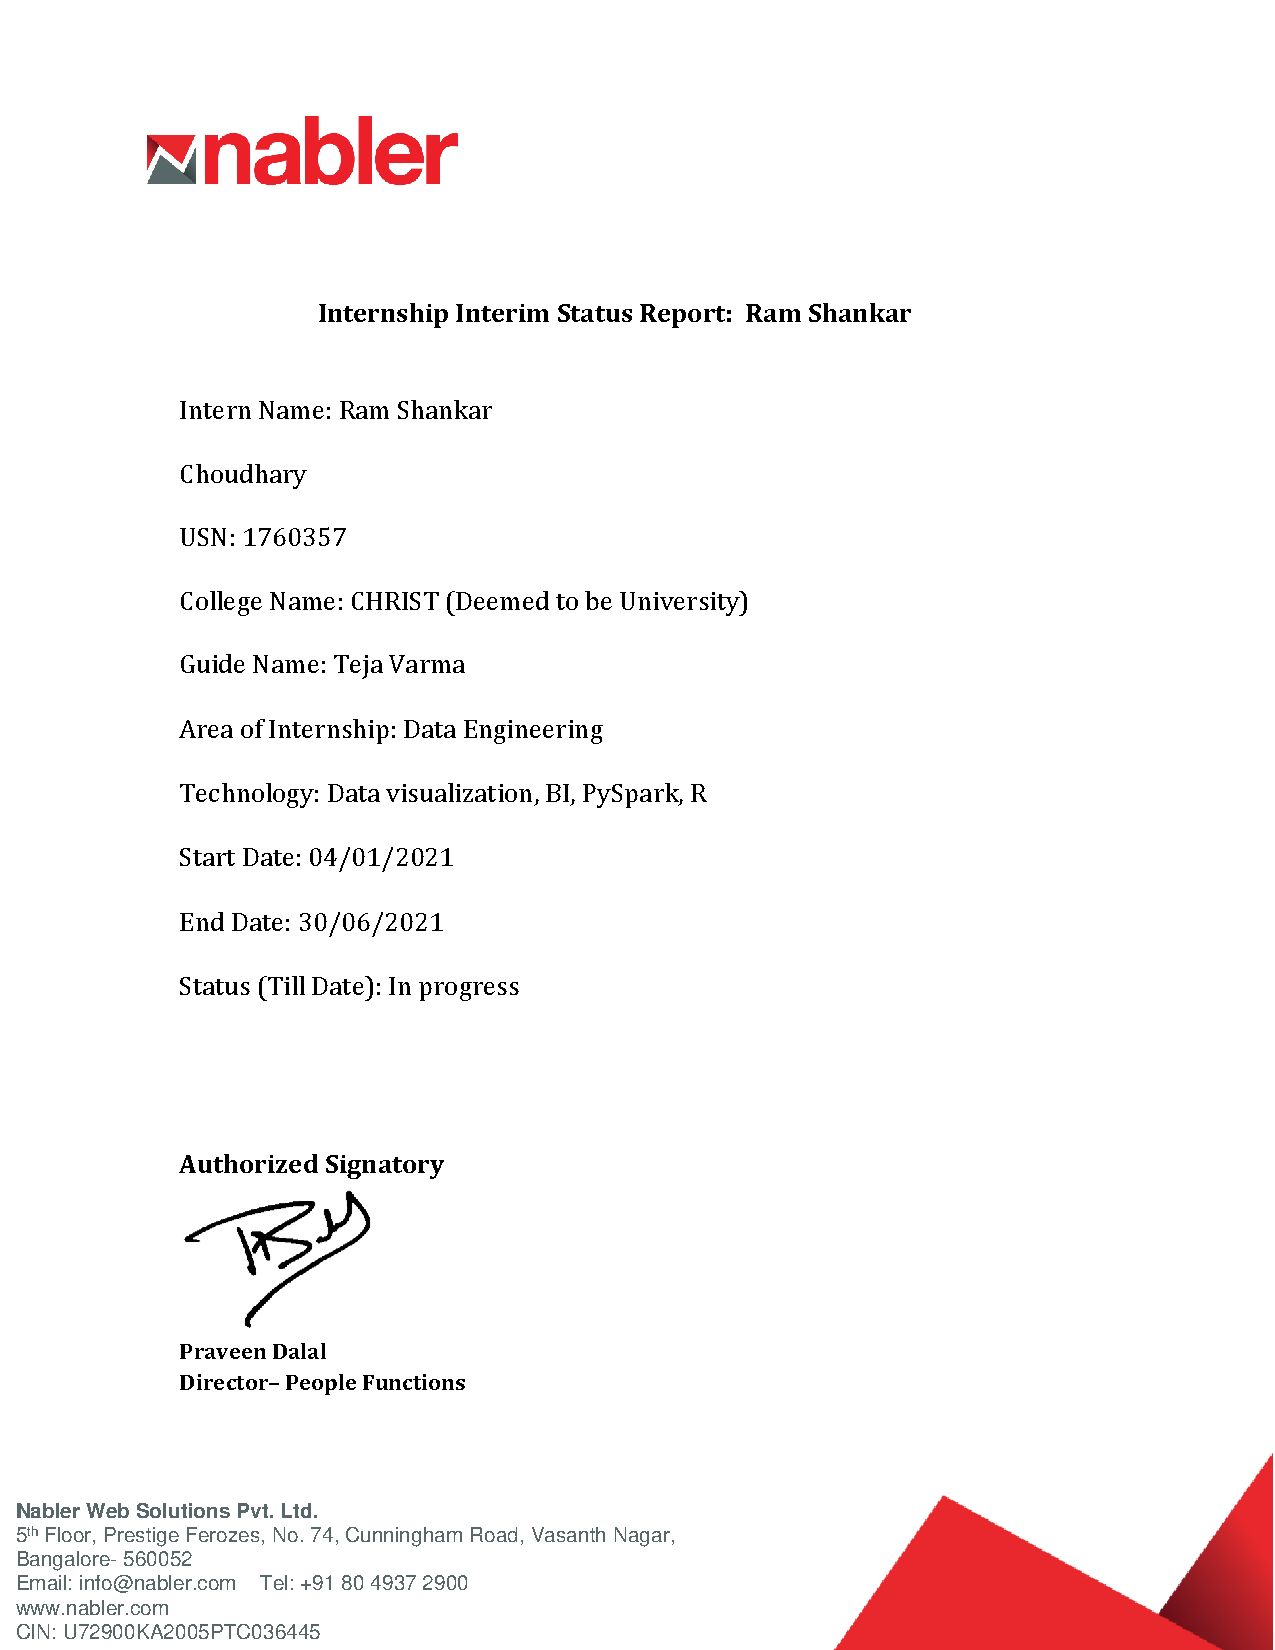
\includegraphics[width=\paperwidth,height=\paperheight]{IndustryCertificate.pdf}
			\end{center}
		\end{figure}
		
	\end{center}
}

\clearpage



%----------------------------------------------------------------------------------------
%	ACKNOWLEDGEMENTS
%----------------------------------------------------------------------------------------

\newpage
\setstretch{1.3} % Reset the line-spacing to 1.3 for body text (if it has changed)

\acknowledgements{\addtocontents{toc}{\vspace{1em}} % Add a gap in the Contents, for aesthetics

\WeorI~would like to thank \textbf{\VCName}, Vice Chancellor,  \UniversityName, \textbf{\ProVCName}, Pro Vice Chancellor, \textbf{\DirectorName}, Director, \CollegeName~and  \textbf{\DeanName}, Dean for their kind patronage. \\

\WeorI~would also like to express sincere gratitude and appreciation to ~\textbf{\HODorCoordinator}, \HODorCoordinatorDesignation,~\DepartmentName~for giving me this opportunity to take up this project. \\

\AcknowledgementForGuide  \\

\ifdefempty{\CoGuideName}{}{\AcknowledgementForCoGuide \\}

\AcknowledgementForOthers \\

%\begin{flushright}
%	\AuthorNameOne,\\
%	\AuthorNameTwo, \\
%	\AuthorNameThree,\\
%	\AuthorNameFour	
%\end{flushright}
}

\clearpage % Start a new page


%----------------------------------------------------------------------------------------
%	DECLARATION PAGE
%----------------------------------------------------------------------------------------

\Declaration{

	
	\WeorI, hereby declare that the project titled~\textquotedblleft\textbf{\ProjectTitleTwo}\textquotedblright~is a record of original project work undertaken for the award of the degree of \textbf{\ProgramName}~in~\textbf{\DepartmentName}. \WeorI~have completed this study under the supervision of \textbf{\GuideName}, \GuideDepartment~\ifdefempty{\CoGuideName}{}{and \textbf{\CoGuideName}, \CoGuideDepartment}.
	
	\WeorI~also declare that this project report has not been submitted for the award of any degree, diploma, associate ship, fellowship or other title anywhere else. It has not been sent for any publication or presentation purpose.
	
	\textbf{Place:} \CollegeName, \\ $~~~~~~~~~~~~~$\UniversityName, \\
	$~~~~~~~~~~~~~$Bengaluru 
	
	\textbf{Date:} \DateofDeclaration
	
	\begin{center}
		\begin{tabular}{ccp{5cm}}
			\hline
			{\large{\textrm{\textbf{Name}}}} & {\large{~\textbf{Register Number}}}
			&{\large{~\textbf{~~~~~~~~~~~~Signature}}}\\
			\hline
			&&\\
			{\large{\textrm{\textbf{\AuthorNameOne}}}} & {\large{~\RegisterNoOne}} &\\
			&&\\
			{\large{\textrm{\textbf{\AuthorNameTwo}}}} & {\large{~\RegisterNoTwo}} &\\
			&&\\
			{\large{\textrm{\textbf{\AuthorNameThree}}}} & {\large{~\RegisterNoThree}} &\\
			&&\\
			{\large{\textrm{\textbf{\AuthorNameFour}}}} & {\large{~\RegisterNoFour}} &\\
			&&\\

		\end{tabular}
	\end{center}
}


\clearpage % Start a new page


%----------------------------------------------------------------------------------------
%	QUOTATION PAGE
%----------------------------------------------------------------------------------------

% \input{Primitives/Quotation}


%----------------------------------------------------------------------------------------
%	ABSTRACT PAGE
%----------------------------------------------------------------------------------------

\abstract{\addtocontents{toc}{\vspace{1em}} 
	
	The use of internet has had many positive effects on education. It has provided us with the means to educate each and everyone without any discrimination, and any limitations (term relative only in terms of education, not the accessibilty limitation). I t overcomes both the limitations that students mostly have, which is time and the amount of space required for various books. This also benefits the teachers who have vast access to all the information and resources from the internet.
	\\
	2020 was the year that challenged all the education systems to re-think the way students could be educated and also resulted in many educational conferences being cancelled. But this also led us to switching to new ideas/processes using internet as the backbone of all the work we do. My project also involved converting an offline exhibition that was held every year to an online variant. 
	\\
	This exhibition has been converted to an online variant wherein scientists, researchers, and scholars from various universities come in and explain about their research and the impact that it produces in real-world. The design and development of the website took nearly 7 months comprising various applications, technolgies, illustrators, animators...etc. For the wireframing and the prototype of the website Adobe XD was the most used application other than Figma and Framer X. The front-end of the website was build using ReactJs framework, using Tailwind-Css, Twin Macro and Styled-Components to style the website. The data is being populated using Google Sheets API as they wanted to quickly keep changing content and wanted that to be reflected in the website without the hassle of updating it constantly to a database like postgres or Mongo as that would also introduce a curve to learn for the non-technical people who were managing the exhibition. The website was put into production using Nginx using the on-site servers. 
	
	}

\textbf{\textit{Keywords}:} React.js, Tailwind, Nginx, Google Sheet API, Git

\clearpage % Start a new page




%----------------------------------------------------------------------------------------
%	LIST OF CONTENTS/FIGURES/TABLES PAGES
%----------------------------------------------------------------------------------------

\pagestyle{fancy} % The page style headers have been "empty" all this time, now use the "fancy" headers as defined before to bring them back

\tableofcontents % Write out the Table of Contents


\lhead{\emph{List of Figures}} % Set the left side page header to "List of Figures"
\listoffigures % Write out the List of Figures

\lhead{\emph{List of Tables}} % Set the left side page header to "List of Tables"
\listoftables % Write out the List of Tables


%----------------------------------------------------------------------------------------
%	GLosarry
%----------------------------------------------------------------------------------------

\clearpage % Start a new page

\glossarylist{

\setstretch{1.5} % Set the line spacing to 1.5, this makes the following tables easier to read
. 

		\begin{tabular}{lp{11cm}}
			\hline
			\textbf{Item} & \textbf{Description}\\
			\hline
			\textbf{Adobe XD} & Adobe XD is a vector-based user experience design tool for web apps and mobile apps, developed and published by Adobe Inc. \\
			
			\textbf{Figma} & Figma is a vector graphics editor and prototyping tool. \\

			\textbf{Framer X} & Framer X is another prototyping tool but with a lot of emphasis on motion design. \\
			
			\textbf{ReactJs} & React is an open-source, front end, JavaScript library for building user interfaces or UI components. \\
			
			\textbf{TailwindCSS} & A utility-first CSS framework packed with CSS classes. \\
			
			\textbf{API} & \textbf{A}pplication \textbf{P}rogramming \textbf{I}nterface \\
			
			\textbf{Nginx} & NginX is a web server that can also be used as a reverse proxy, load balancer, mail proxy and HTTP cache.  \\
			
			\hline
		\end{tabular}
		
}


%----------------------------------------------------------------------------------------
%	THESIS CONTENT - CHAPTERS
%----------------------------------------------------------------------------------------

\mainmatter % Begin numeric (1,2,3...) page numbering

\pagestyle{fancy} % Return the page headers back to the "fancy" style

% Include the chapters of the thesis as separate files from the Chapters folder
% Uncomment the lines as you write the chapters

\fancyhead[]{}
%\fancyhead[CO]{\ProjectTitle}
%\fancyfoot[CO]{\DepartmentName, \\ \CollegeName}
%\fancyfoot[CO]{\hline}
\renewcommand\footrulewidth{0pt}
\renewcommand\headrulewidth{0pt}
\fancyfoot[R]{\thepage}


\chapter{INTRODUCTION} % Main chapter title
\label{ChapterIntroduction} % For referencing the chapter elsewhere, use \ref{ChapterIntroduction} 



The techonology has evolved rapidly and providede us with various ways to communicate on a global scale and assess vast amopunt of information with a click. This benefit can be utilized by various sectors, and one of them is education which can can greatly be made more efficient by removing limitations of time, space and money. Students could watch a topic being thought any time of the day, anywhere and also maybe for free of cost. With the rise of pandmic, and with the restrictions to the people, the technology to teach people has gathered a lot of attention and all the educational institutions are implementing various ways using these technologies. This is the same for organizing various educational events which hel pstudents learn much more than their syllabus and provides them a way to essentially choose their career path. My project also is invovled in developing such a website that is used to educate students with a very minimal user experience, so as to let all the age groups be able to access the website.
\\
The purpose of this project was to implement an approach of user experience for a website design, that could highlight all the events conducted in the exhibition that also brought about the vision the client i.e Ajith wanted it to be, and also to develop this using the necessary technologies. While wrking on this project I mostly 
concentrated on revealing and understanding the concepts of UX design which include usability, visual design and human factors affecting the user experience.
The vision that the client wanted wanted was for the website to look simple and yet elegant and to be accessible on any device without any hiccups with great user experience. With a lot of thinking, wireframing, and prototyping we came up with a design and a story that would be narrated by a host while show-casing the website.
The process of designing and developing was divided into various phases like wireframing, designing, prototyping, data gathering, developing front-end, connecting APIs, and the deploying to an in-house server.   


\section{Problem Formulation}
Under this the reason for choosing the particular problem or title for the project shall be explained along with the thought process that was involved in doing so.
Since this project was for an online exhibition, the main goal was for it to have a very nice user experience, and also to tell a story from the narrator's point of view during the event.
My aim was to understand all the design aesthetics needed for the project, and for that I needed to clearly undestand the scope of this exhibition as this would help me imagine and approach the design as intended by the narrator of the website(i.e the host of the online exhibition).
The user experience and and the libraries that will be used to complete this project would be a problem as everything would have to be customized as the client would want it to be.

\section{Problem Identification}

Clearly, the problem here would be designing a good user experience that bodes well for people of all ages and provides them with a intriguing experience to enjoy the whole exhibition, along with the narrator. User experience concentrates on how the overall design makes the user to feel. To create not just beautiful but also qualitative and well-worked design is why a user experience design is needed. To achieve positive user feelings during using a website, designers should understand users’ goals, desires, fears, behaviors and ambitions. The problem during software development is that the technical approaches/practices are more popular than user-centric ones. Based on a huge number of surveys conducted by the groups with strong reputation in software production, this is a problem which leads to unsuccessful projects. The reason is the lack of attention to user inputs. In the website design the user experience is identified by not just usability alone. It's also impacted by a lot of design components that UX design covers. It includes usability, utility, design, human factors, accessibility, persuasiveness and others. All these factors while designing also afftect the way that a website has to be developed, because the layout needs to be as accurate to the design as possible.


\section{Problem Statement \& Objectives}
The project is meant to design and develop a website that has a good user experience, that can be used by people of all ages without much effort. It should be responsive and visually pleasing pleasing to all kinds of user. 
This website if for an exhibition that is being converted to an online exhibit and needs a lot of design approaches to be used to make it like so.

\section{Limitations}

There are a few limitations regards to this project alone, as I am the only developer who would also design the user experience of the online exhibit and due to the team not being technaical various terminology issues arise, where I have to summarize what I mean, and also the lack of understanding of the domains of which the exhibit is conducted presents an issue by itself. Technically, there is one limitation I would like to highlight; which is not using a database but rather a google sheet api which is not a good approach, but it was done due to the limitation of team not being being technically adept and also because it would reduce my(developer's) burden to constantly keep updating data. 

\chapter{RESEARCH METHODOLOGY} 
\label{ChapterResearchMethodology} 
% For referencing the chapter elsewhere, use \ref{ChapterResearchMethodology} 


Research methodology is defined as a systematic study of defining a problem and formulating a hypothesis by collecting and analyzing data and information and making deductions and conclusions based on it. Research is often considered as a careful investigation or inquiry specifically through search for new facts in any branch of knowledge. Its main purpose is to inform action, to prove a theory, and contribute to developing knowledge in a field or study. In prior to developing any project or product,company firstly conducts a thorough research on demanded product its going to develop, whether or not it is scalable for all clients, how much will it benefit them; what are the advantages and shortcomings of existing systems One of main concern is how we can overcome them to create a more advanced, simple, interactive and easy-to-use system for both employers and employees. In my case, the problem lies in the design and the modeling of the website and how it needs to be implemented. This website is made to emulate an exhibition and has been converted to an online variant wherein scientists, researchers, and scholars from various universities come in and explain about their research and the impact that it produces in real-world.

		



 

\chapter{LITERATURE SURVEY AND REVIEW} % Main chapter title
\label{ChapterLiteratureSurvey} % For referencing the chapter elsewhere, use \ref{Chapter1} 

Any research based project is incomplete without a literature survey and review. Hence, this chapter is mandatory to both MTech and BTech projects. This chapter is mainly divided into two sub-chapters. Namely:
\begin{itemize}
	\item Literature collection and segregation (called as literature survey – collection of data)
	\item Critical review of selected literature (from the ones collected during the survey)	
\end{itemize}

The first cub-chapter is very straight forward to understand and perform. However, more emphasis is given to the second sub-chapter – Critical review. Consult with your guides/supervisors to understand this aspect and complete it accordingly. A slideshare presentation on literature review is a recommended reading. 

\section{Literature Collection \& Segregation}


\section{Critical Review of Literature}


\chapter{ACTUAL WORK} % Main chapter title
\label{ChapterActualWork} % For referencing the chapter elsewhere, use \ref{Chapter1} 


Upon completion of identifying \& formulating the research problem, and carrying out the necessary literature survey and review, the actual work on the project is taken-up. This chapter is dedicated to the actual work done by students. Hence, the chapter name and sub-chapter names are not fixed. It is left to the discretion of the students with appropriate guidance from their respective supervisors. However, one or more of the following aspects (as applicable) shall be covered in this chapter:
\begin{itemize}
	\item Methodology of the study or actual work (different from research methodology)
	\item Experimental and/or analytical work completed in the project
	\item Modeling, Analysis and Design
	\item Prototype and testing
\end{itemize}

In this project, I help design and build a web-site that is visually pleasing to all the age groups and has a great user experience. This website is designed to emulate how an offline exhibit would be like. A lot of work went into the design and the user experience of the website, and then more during web development. Various applications, and web-development technologies were utilized to create this online exhibit. 

% \Section{Software Requirements}\index{Software Requirements}

Software Requirements
\\
\textbf{Adobe XD}
Adobe XD is a vector-based digital design tool for websites and apps. It is used to  create and collaborate on everything from prototypes to mockups to full designs. It is developed by Adobe and is available for Windows and macOS. It supports website, mobile, apps,etc to create wireframes and click-through prototypes.


\textbf{Framer X}

\textbf{React Js}

\textbf{Tailwind CSS}

\textbf{ Frame Motion }

\textbf{Google Sheet API}

\textbf{React Slick - used in creating the custom slider}






\section{Methodology for the Study}\index{Methodology}

The purpose of creating a website for the online exhibition is to provide a medium for students, researchers, and scholars to gather and get to know about the research of various other scientists/researchers from various other fields. The first step to do that is to make the website have a very good user experience and that can be used by all age groups, and also make is simple yet elegant in the views of these users. This is done by a lot reserach of the way the various interactionms can be shown and also the best way to show details of a particular exhibit. 

\section{Experimental and or Analytical Work Completed in the Project}

\textbf{Using React Slick to create a custom slider}
\\
React slick is a react component that can be used to create custom carousel's based on various parameters and CSS tweaking. React-Slick by itself is a component made up of javascript and css which has a basic slider functionality that we have used in this project to create the main page by customizing it a lot. The reason to choose this project over any other was because of the simplicity and the accessibility to its parent code that is provided to us when we install it. 

\textbf{Google Sheets API}
\\
Google sheets API provides us a way to Read, write, and format data in Sheets using the their API. This API has a lot of settings with which we can create beautiful and functional sheets within the code itself. Each spreadsheet has an id associated to it(you can also have a look at this id in the url when you open a google spreadsheet).
The main reason we choose this API was to read the cells of the spreadsheet, so that data from here can be populated in the exhibition website.  

\section{Modeling, Analysis \& Design}

\section{Prototype \& testing}

\section*{Sample LaTeX Typesetting}


\paragraph*{Figure} Vector Graphics EPS Format [Figure \ref{fig:fcmc1}]
\begin{figure}[H]
	\begin{center}
		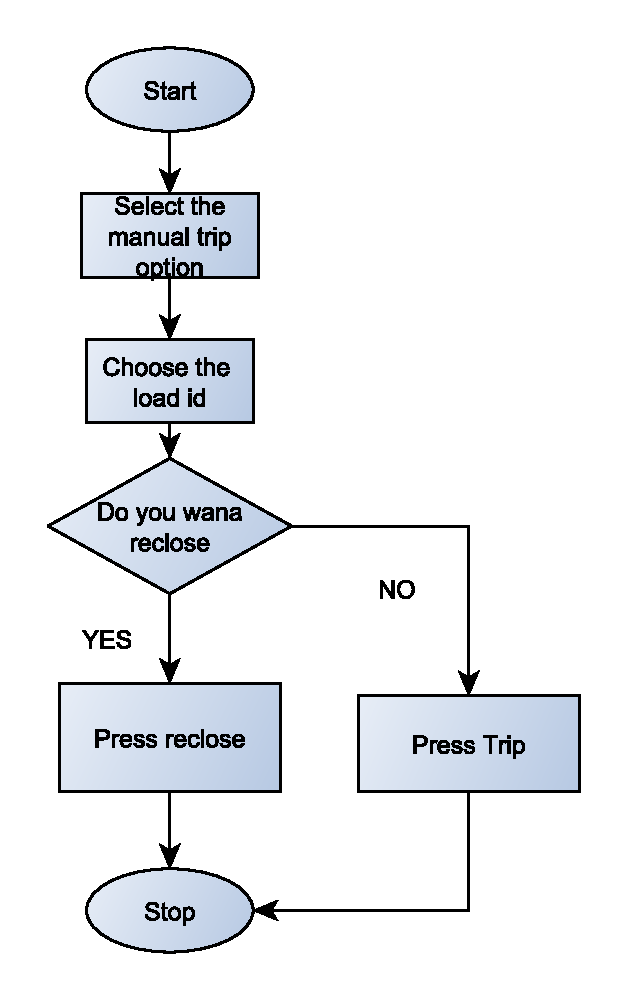
\includegraphics[scale=0.5]{Figures/manualtrip.eps}
		\caption{Flowchart of Manual Controller}
		\label{fig:fcmc1}
	\end{center}
\end{figure}


\paragraph*{Figure} JPEG/JPG Format [Figure \ref{fig:rb}]
\begin{figure}[h]
	\begin{center}
		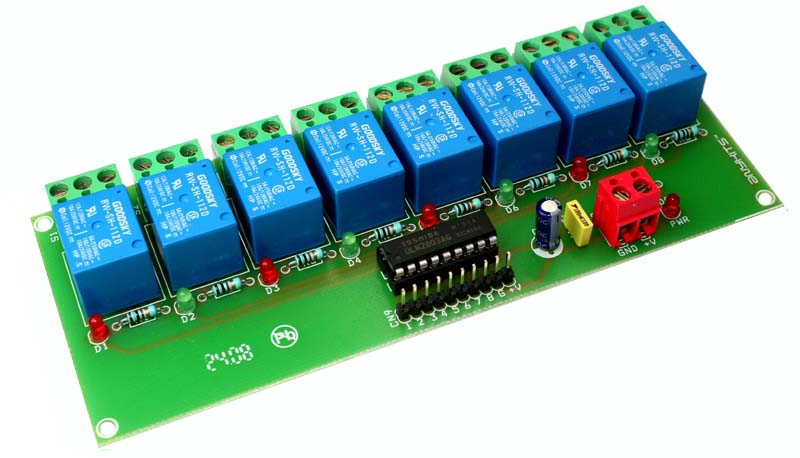
\includegraphics[scale=0.3]{Figures/relay.jpg}
		\caption{Relay Board}
		\label{fig:rb}
	\end{center}
\end{figure}

\paragraph*{Table} Refer [Table \ref{tab:sm}]
\begin{table}[h]
	\centering
	\caption{Student Marks}
	\begin{tabular}{rr}
		\toprule
		Name  & Marks \\
		\midrule
		Ajay  & 10 \\
		Vinay & 20 \\
		\bottomrule
	\end{tabular}%
	\label{tab:sm}%
\end{table}%


\paragraph*{Cross References: Citation, Index, Reference, Equation reference}
This is the methodology for the entire project work which includes even the process of deciding on the project title, objectives
\index{Ojectives}, etc. This is mandatory for MTech and optional for BTech)\cite{abcdef}. The data is shown in Table \ref{tab:sm}. The equation shown in Equation \eqref{Eq:eq123}

\paragraph*{Inline Equation}
This is my equation.
$	f = ma \pm \alpha \Delta \left[ {\begin{array}{*{20}{c}}
	1 & \chi   \\
	{ - 1} & 0  \\
	\end{array}} \right] $
,which is appearing in between some text.

\paragraph*{Equation without Numbering} 
\begin{equation*}
	x = \frac{{ - b \pm \sqrt {{b^2} - 4ac} }}{{2a}}\
\end{equation*}

\paragraph*{Equation with Numbering} 
\begin{equation} \label{Eq:eq123}
\dot X = \left[ {\begin{array}{*{20}{c}}
	1 & p  \\
	2 & \alpha   \\
	\end{array}} \right]\left[ {\begin{array}{*{20}{c}}
	{{x_1}}  \\
	{{x_2}}  \\
	\end{array}} \right] + Bu\
\end{equation}



\paragraph*{Algorithm Format} 
\begin{algorithm}
	\caption{Addition of two 8 bit numbers}\label{alg:add8bit}
	\begin{algorithmic}[1]	
		\\ Start
		\\ Input a and b
		\\ c=a+b
		\\ Output c
		\\ stop
	\end{algorithmic}
\end{algorithm}


\paragraph*{Enumeration Format}
The following are the different flavor of Tex systems
\begin{enumerate}
	\item TeXLive TeX System
		\begin{enumerate}
			\item TeXLive for Windows
			\begin{enumerate}
				\item TeXLive
				\item ProTex
			\end{enumerate}
			\item MacTeX for Mac
		\end{enumerate}
	\item MikTeX TeX System
\end{enumerate}

\paragraph*{Bullets Format}
The following are the advantages of LaTeX,
\begin{itemize}
	\item {\LaTeX} is highly portable and free.
	\begin{itemize}
		\item Contribute to TUG
		\item Promote Free Softwares
	\end{itemize}
	\item Operating-system independent.
	\item Complex scientific documents can be created
	automatically.
	\item High quality math typesetting.
\end{itemize}

\paragraph*{Program Inclusion} Program file present in other directory can be embedded into the report.
\lstinputlisting{Files/code.asm}

\paragraph*{Verbatim Text} Include text as it is.
\\
The additional database schema is shown below which is used to store all the configuration and transaction data.
\begin{verbatim}
CREATE TABLE `controller_config` (
`load_id` int(11) NOT NULL,
`ct_constant` double DEFAULT NULL,
`pt_constant` double DEFAULT NULL,
`samples` int(11) DEFAULT NULL,
`delay` double DEFAULT NULL,
PRIMARY KEY (`load_id`)
) ENGINE=InnoDB DEFAULT CHARSET=utf8;
SELECT * FROM loadcontroller.load_details;
\end{verbatim} 


 
 \chapter{RESULTS, DISCUSSIONS AND CONCLUSIONS} % Main chapter title
\label{ChapterResults} % For referencing the chapter elsewhere, use \ref{Chapter1} 
As every project starts with a goal to establish, a problem to solve and to make existing
projects better, they all lead to a result. These results helps us to determine whether the
approach taken, job done, analysis and research conducted was correct and up to the
mark or not. These results then help us to conclude what we have gained from all the
hassle of researching, developing and testing.

\section{Results \& Analysis}
The website, after several bug fizes and updates, feels very smooth and has good user experience as the client would want it. It is easily able to run both mobile phones and desktops. The following are the highlights of the website.
\\
1. The user experience is simple and elegant such that people of any age will easily be able to go through the website. 
\\
2. The main page with the carousel is gesture friendly, it can be operated via gestures using mouse, hand gestures, touch pens..etc   -
\\
3. Mobile frindly even with a lot animations that have to load up. A lot of optimizations were done to the the gifs before exporting them so that it can easily be loaded on websites.
\\
4. The website is well adapted and tested to handle real time data, with instant changes in Google sheet data. The website automatically updates after a new refresh with the latest data from the google sheet data


\section{Comparative Study}
There are a lot of websites that are used to showcase various educational exhibits, some of the most notable one's are \href{https://firstladies.si.edu/gallery}{First Ladies of United States} and \href{https://www.npg.si.edu/}{National Portrait Gallery}. These were taken as an inspiration to design and develop the exhibition website, but make it more simple and user friendly. After the completion of the development process, here are a few
aspects that stand out from other dashboards:
\\
1. The application is made to look simple and is less straining to one's eye's when the all the focus is given only to the main content.
\\
2. The main page has a custom made carousel that is accessible very easily both on large and smaller screens.
\\
3. All the details come from a live google sheet that is continously being maintained for the latest and most accurate information and latest exhibits.


\section{Discussions}
This project opens up a lot of topics that can be discussed to educate common public, researchers, scholars, and students with various research and studies happening around them. It opens up the possibility to conduct online exhibitions with various other factors that can be included like quizzes, games, competitions..etc on  the internet 

\section{Conclusions}
The completeion of this project led to an online exhibition being called \href{https://cosmic-zoom.in/}{Cosmic-Zoom} held by \href{https://www.icts.res.in/}{ICTS(International Centre for Theoretical Sciences
)}, a centre of the Tata Institute of Fundamental Research which is a research institute which wanted to conduct an exhibition showcasing their research and scienctific discoveries in a storified manner through the website. 
This project led me to learn a lot of technoilogies and many Javascript libraries like react-router, styled-components, twin macro, framer motion and many many more. It also helped me look websites from a new perspective, of a designer as to how the user experience of a user can be increased and all components that are attached to this.


\section{Scope for Future Work}

1. Using a CDN to get the files and store in the user's cache is much better than loading it up at each reload
2. It is better to get data from a database rather than using Google Sheet API to get data from. The easy solution to this is to build an admin page that has access to the database, and has an editor like \href{https://quilljs.com/}{Quill.js} to be able to edit all the data, which will update on the website too.
3. More image optimization has to be done to let the image lazy-load only after all the other UI components and text have successfully loaded. This'll make it faster to browse the site from one page to the other very quickly.
 



	
	






 

\addtocontents{toc}{\vspace{2em}} % Add a gap in the Contents, for aesthetics



%----------------------------------------------------------------------------------------
%	BIBLIOGRAPHY
%----------------------------------------------------------------------------------------


%\label{Bibliography}

%\lhead{\emph{Bibliography}} % Change the page header to say "Bibliography"

\bibliographystyle{unsrtnat} % Use the "unsrtnat" BibTeX style for formatting the Bibliography
%
%\bibliography{Bibliography} % The references (bibliography) information are stored in the file named "Bibliography.bib"
\addtotoc{BIBLIOGRAPHY}

\begin{thebibliography}{1}

% New edition of a book

\bibitem{BanksPorcello}
Hartson R, Pyla PS,\emph{The UX Book: Process and guidelines for ensuring a quality user experience} Elsevier, 2012 Jan 25.

\bibitem{Kalfatovic}
Kalfatovic MR, Creating a winning online exhibition: A guide for libraries, archives, and museums. American Library Association, 2002.

\bibitem{m}
Lester P. Is the virtual exhibition the natural successor to the physical?. Journal of the Society of Archivists, 2006 Apr 1

\bibitem{n}
Khoon LC, Ramaiah CK, Foo S. The design and development of an online exhibition for heritage information awareness in Singapore. Program. 2003 Jun 1.

\bibitem{BanksPorcello}
Banks A, Porcello E, \emph{Learning React: functional web development with React and Redux}, OReilly Media, Inc. 2017 Apr 27.

\bibitem{a}
Kelly C. Guidelines for designing a good website for ESL students. The internet TESL journal. 2000 Mar;6(3):1-9.

\bibitem{b}
van de Laar B, Bos DP, Reuderink B, Poel M, Nijholt A. How much control is enough? Influence of unreliable input on user experience. IEEE transactions on cybernetics. 2013 Oct 1;43(6):1584-92.

\bibitem{d}
Garrett JJ. The elements of user experience: user-centered design for the web and beyond. Pearson Education; 2010 Dec 16.

\bibitem{e}
Agarwal A, Meyer A. Beyond usability: evaluating emotional response as an integral part of the user experience. InCHI'09 Extended Abstracts on Human Factors in Computing Systems 2009 Apr 4 (pp. 2919-2930).

\bibitem{f}
Kalbach J. Designing Web navigation: Optimizing the user experience. OReilly Media, 2007 Aug 28.

\bibitem{g}
Sutcliffe A, Hart J. Analyzing the role of interactivity in user experience. International Journal of Human–Computer Interaction. 2017 Mar 4


\bibitem{React}
Fedosejev A. React. js essentials. Packt Publishing Ltd; 2015 Aug 27.


\bibitem{h}
Vipul AM, Sonpatki P. ReactJS by Example-Building Modern Web Applications with React. Packt Publishing Ltd; 2016 Apr 21.

\bibitem{i}
Khalili A, Loizou A, van Harmelen F. Adaptive linked data-driven web components: Building flexible and reusable semantic web interfaces. InEuropean semantic web conference 2016 May 29 (pp. 677-692). Springer, Cham.

\bibitem{j}
Javeed A. Performance optimization techniques for reactjs. In2019 IEEE International Conference on Electrical, Computer and Communication Technologies (ICECCT) 2019 Feb 20 (pp. 1-5). IEEE.

\bibitem{k}
Alawar MW, Abu-Naser SS. CSS-Tutor: An intelligent tutoring system for CSS and HTML.

\bibitem{l}
Robson E, Freeman E, Head First Html With CSS and XHTML, OReilly Media, 2005 Dec 8.



% CONTENT BELOW IS FROM TEMPLATE

% \bibitem{BrusawAired}
% C. Brusaw, C. Aired, and W. Oliu, \emph{Handbook of Technical Writing}, 3rd ed. New York: St. Martin’s Press, 1987.

% \bibitem{abcdef}
% S.K. Kenue and J.F. Greenleaf, “Limited angle multifrequency diffiaction tomography,” \emph{IEEE Trans. Sonics Ultrason}., vol. SU-29, no. 6, pp. 213-2 17, July 1982.

% % Book
% \bibitem{MorseFeshback}
% P.M. Morse and H. Feshback, \emph{Methods of Theoretical Physics}. New York: McGraw Hill, 1953.

% % Journal Article
% \bibitem{KenueGreenleaf}
% S.K. Kenue and J.F. Greenleaf, “Limited angle multifrequency diffiaction tomography,” \emph{IEEE Trans. Sonics Ultrason}., vol. SU-29, no. 6, pp. 213-2 17, July 1982.


% \bibitem{abcd}
% M.M. Botvinnik, \emph{Computers in Chess: Solving Inexact Search Problems}. Translated by A. Brown, Berlin: Springer-Verlap, 1984.

% % Article in an Anthology
% \bibitem{Broadhead}
% G.J. Broadhead, “Style in technical and scientific writing.” In M.G. Moran and D.Joumet, eds. \emph{Research in Technical Communication. A Bibliographic Sourcebook}, pp. 379-401. Westport. CT: Greenwood Press, 1985.

% % Translation
% \bibitem{Botvinnik}
% M.M. Botvinnik, \emph{Computers in Chess: Solving Inexact Search Problems}. Translated by A. Brown, Berlin: Springer-Verlap, 1984.

% % Personal Interview/Communication
% \bibitem{Elmer}
% Interview [or Personal Communication] with Prof. Elmer Hixon, BCE Department, The University of Texas at Austin, March 12, 1995.

% % Handbook/date book, no author
% \bibitem{Washington}
% \emph{Handbook for Writing Operation and Maintenance Manuals.} Washington, D.C.: Packaging Machinery Manufacturers Institute, 1973.

% \bibitem{Austin}
% \emph{Interface Circuits Data Book}, Texas Instruments, Austin, Texas, 1993.

% \bibitem{Microsoft}
% \emph{User’s Guide: Microsoft Word,} Vers. 5.0, Microsoft, 1991.

% % Encyclopedia Entry

% % No author given:
% \bibitem{Brittanica}
% “Sonar,” \emph{Encyclopaedia Brittanica}, 1984 ed.

% % Author(s) given:
% \bibitem{PearsonMacChesney}
% A.D. Pearson, J.B. MacChesney, and W.G. French, “Fiber optics,” in \emph{Encyclopedia of Semiconductor Technology}, M. Grayson, Ed., New York: John Wiley \& Sons, 1984.

% % Online:
% \bibitem{BrittanicaOnline}
% “Greyhound,” \emph{Brittanica Online}, Beta Version 96.1, March 1996.

% % Course Notes
% \bibitem{Jones}
% J. K. Jones, \emph{Lab Notes for EE464K, Senior Projects}, The University of Texas at Austin, fall semester, 1994.

% % Dissertation or thesis
% \bibitem{Tsikos}
% B. Tsikos, “Segmentation of 3-D scenes using multi-modal interaction between machine vision and programmable mechanical scene manipulation,” Ph.D.
% dissertation, Univ. of Pennsylvania, BCE Dept., Philadelphia, 1987.

% % Proceedings paper
% \bibitem{Finkel}
% R. Finkel, R. Taylor, R. Bolles, R. Paul, and J. Feldman, “An overview of AL, programming system for automation,” in \emph{Proc. Fourth Int. Joint Conf Artif. Intell.}, pp. 758-765, Sept. 3-7, 1975.

% % Patent
% \bibitem{Norman}
% L.O. Norman, U.S. Patent 4 379 752, 1983. [Title of patent may be included.]

% % Newspaper article
% \bibitem{Wall}
% “Technology threatens to shatter the world of college textbooks, \emph{The Wall Street Journal}, vol 91, pp. Al, A8, June 1, 1993.

% % Government publication
% \bibitem{Wall}
% \emph{Basic Facts about Patents}. Washington, D.C.: Government Printing Office, 1989.

% % Technical Report
% \bibitem{CoxTurner}
% R. Cox and J. S. Turner, “Project Zeus: design of a broadband network and its
% application on a university campus,” Washington Univ., Dept. of Comp. Sci.,
% Technical Report WUCS-91-45, July 30, 1991.


% % Letter/E-mail
% \bibitem{Beck}
% Letter from J. M. Beck, Project Manager, TI, Bedford, Utah, Sept. 3, 1996.

% % Software
% \bibitem{Janzen}
% M. Janzen, \emph{Instant Access Accounting}. Computer software. Nexus Software, Inc IBM-PC, 1993.


% % Electronic bulletin board
% \bibitem{AIDS}
% AIDS Info BBS. [San Francisco (CA): Ron Gardner]. Available from: 415-626-1246.

% % Database/online
% \bibitem{Duncan}
% R. Duncan, “An HTML primer,” \emph{PC Magazine}, June 13, 1995, v14, n11 p. 261(7) in Academic Index (database on UTCAT PLUS system).

% \bibitem{Berdan}
% R. Berdan and M. Garcia, \emph{Discourse-Sensitive Measurement of Language Development in Bilingual Children} (Los Alamitos, CA: National Center for
% Bilingual Research, 1982) (ERIC ED 234 636).

% % World Wide Web (give author and title if named)
% \bibitem{Fuminao}
% Fuminao Okumura and Hajime Takagi, “Maglev Guideway On the Yamanashi Test Line,” \emph{http://www.rtri.or.jp/rd/maglev2/okumura.html,} October 24, 1998.

% \bibitem{Supplies}
% “AT\&T Supplies First CDMA Cellular System in Indonesia,” \emph{http://www.att.com/press/1095/951011.nsa.html}, Feb 5, 1996.

\end{thebibliography}  


%\backmatter
\clearpage % Start a new page

%\chapter{Publication Details}

\publicationlist{
%\label{PublicationDetails}

%\lhead{\emph{Publication Details}}
\justify

S.K. Kenue and J.F. Greenleaf, “Limited angle multifrequency diffiaction tomography,” \emph{IEEE Trans. Sonics Ultrason}., vol. SU-29, no. 6, pp. 213-2 17, July 1982.

}

\pagebreak




%----------------------------------------------------------------------------------------
%	THESIS CONTENT - APPENDICES
%----------------------------------------------------------------------------------------

\addtocontents{toc}{\vspace{2em}} % Add a gap in the Contents, for aesthetics

\appendix % Cue to tell LaTeX that the following 'chapters' are Appendices

% Include the appendices of the thesis as separate files from the Appendices folder
% Uncomment the lines as you write the Appendices

% Appendix A

\chapter{Appendix A Title} % Main appendix title
\label{AppendixA} % For referencing this appendix elsewhere, use \ref{AppendixA}

Since the chapters are numerically numbered, the appendices shall be numbered using alphabets (English capital letters). The items that can be inserted as appendices are (list is not exhaustive):

\begin{itemize}
	\item Project synopsis or proposal (if submitted before starting the project)
	\item Photos
	\item Software model analysis reports (these shall not be inserted in the main body of the report)
	\item Project schedules
	\item Selected material from the data collected
	\item Miscellaneous analysis and reports
\end{itemize}


\section{Appendix A Section 1}

\subsection{Appendix A Subsection for Section 1}

\section{Appendix A Section 2}
% Appendix B

\chapter{Custom Carousel} % Main appendix title
\label{AppendixB} % For referencing this appendix elsewhere, use \ref{AppendixA}


A customized carousel was built by me for the main poage of the exhibit to implement the design that we had created. The carousel was created using the help of a library called React-Slick, which is a slider library that also let's you customize it's parameter's through javascript, and CSS(Cascading Style Sheets). 
For the website to be as the client wanted i.e to be accessible by any age groups, a lot of thought went into how the inputs would affect the slider, and how it would scale in different devices. Below is an example of the Carousel component built using React with dummy data.

\lstinputlisting{Files/customCarousel.js}

Below is the custom CSS used for the aove React component
\lstinputlisting{Files/customCarousel.css}


Since space is a factor while creating a report, here is a link to \href{https://gist.github.com/BlankRiser/f904353998562ae974735a561ed9cfb2}{Custom Carousel Gist} which has full data(only needs the gifs, but not shareable due to restrictions)




%----------------------------------------------------------------------------------------
%	Index Page
%----------------------------------------------------------------------------------------
\printindex

\end{document}  